%!TEX root = ../main.tex
%%%%%%%%%%%%%%%%%%%%%%%%%%%%%%%%%%%%%%%%%
%
%LEZIONE 27/09/2016 - PRIMA SETTIMANA (1)
%
%%%%%%%%%%%%%%%%%%%%%%%%%%%%%%%%%%%%%%%%%
\chapter{Proprietà elementari delle funzioni olomorfe}

Rivediamo alcune nozioni basilari dei numeri complessi, andando in particolare a descrivere la relazione che intercorre fra \(\C\) e \(\R^2\).

Come prima cosa ricordiamo che \(\R^2\) è un'\emph{algebra}\graffito{un algebra è uno spazio vettoriale con una struttura di prodotto} con il seguente prodotto:
\[
	(x,y)(x',y') = (x\,x' - y\,y', y\,x' + x\,y').
\]
In \(\C\) questo prodotto può essere facilmente espresso con la notazione comune
\[
	(x+i\,y)(x'+i\,y') = (x\,x'-y\,y') + i\,(y\,x'+x\,y').
\]

Ricordiamo che la norma di \(z\in\C\) è definita come segue
\[
	\abs{z} = \sqrt{z\,\conj{z}},
\]
ovvero, se \(z=x+i\,y\),
\[
	\abs{x+i\,y} = \sqrt{(x+i\,y)(x-i\,y)} = \sqrt{x^2+y^2} = \norma{(x,y)}.
\]
Grazie alla notazione introdotta all'inizio, è facile mostrare che la norma del prodotto complesso è uguale al prodotto delle norme.
Infatti:
\[
	\abs{(x,y)(x',y')} = \abs{(x,y)}\abs{(x',y')}.
\]

Un numero complesso può essere rappresentato in diverse maniere.
Una delle più comuni è la rappresentazione sul \emph{piano di Argand}, la quale sfrutta la relazione fra \(\R^2\) e \(\C\) che fra poco andremo a dimostrare.
Essa associa al numero complesso \(z=x+i\,y\) il punto \((x,y)\) sul piano cartesiano.

Un'altra celebre rappresentazione dei numeri complessi, detta \emph{rappresentazione polare di Gauss}, sfrutta la possibilità di individuare un punto sul piano cartesiano tramite coordinate polari in maniera univoca:
\[
	z = \r\,e^{i\,\q}, \qquad\text{con }\r=\abs{z} \quad\text{e}\quad \q = \arg{z}.
\]
Da questa notazione è possibile intuire che alla moltiplicazione in \(\C\) è associata una roto-dilatazione in \(\R^2\).
Ovvero, preso un numero complesso \(\a\in\C\), vi è associato il seguente operatore lineare:
\[
	M_\a\colon \C \to \C, z\mapsto z\cdot\a.
\]
Tramite la rappresentazione polare, se \(\a = \r\,e^{i\,\q}\) e \(z=\tilde{\r}\,e^{i\,\tilde{\q}}\), si ha
\[
	M_\a\colon \tilde{\r}\,e^{i\,\tilde{\q}} \mapsto \r\,\tilde{\r}\,e^{i\,(\q+\tilde{\q})}.
\]
Ad esempio se \(\a=e^{i\,\pi/3}\), allora \(M_\a\) è una rotazione di \(\frac{\pi}{3}\).

Mostriamo ora la corrispondenza biunivoca fra \(\R^2\) e \(\C\) in maniera formale.
Definiamo quindi la seguente applicazione:
\[
	j\colon \R^2 \to \C, \begin{pmatrix}x\\y\end{pmatrix} \mapsto x+i\,y.
\]
Se adesso consideriamo l'operatore lineare della moltiplicazione \(M_\a\), deve necessariamente esistere una matrice \(A\) tale che il seguente diagramma commuti:
\[
	\begin{tikzcd}
		\C \arrow{r}{M_\a} & \C\\
		\R^2 \arrow{u}{j} \arrow[swap]{r}{A} & \R^2 \arrow[swap]{u}{j}
	\end{tikzcd}
\]
Per quanto detto, sappiamo già che la matrice deve corrispondere ad una roto-dilatazione.
Per trovarla esplicitamente assumiamo che il diagramma commuti, avremo:
\[
	A = j^{-1} M_\a\,j,
\]
posto \(\a = a+i\,b\), segue
\[
	\begin{split}
		A \begin{pmatrix}x\\y\end{pmatrix} & = j^{-1}M_\a\,j \begin{pmatrix}x\\y\end{pmatrix} = j^{-1} M_\a (x+i\,y) = j^{-1} \big[\a(x+i\,y)\big]\\
		& = j^{-1}\big[(a\,x-b\,y)+i(a\,y+b\,x)\big] = \begin{pmatrix}a\,x-b\,y\\a\,y+b\,x\end{pmatrix}\\
		& = \begin{pmatrix}a & -b\\b & a\end{pmatrix} \begin{pmatrix}x\\y\end{pmatrix}.
	\end{split}
\]
Da cui
\[
	A = \sqrt{a^2+b^2} 		\begin{pmatrix}
		\frac{a}{\sqrt{a^2+b^2}} & -\frac{b}{\sqrt{a^2+b^2}} \\[0.3em]
		\frac{b}{\sqrt{a^2+b^2}} & \frac{a}{\sqrt{a^2+b^2}}
	\end{pmatrix}
	= \sqrt{a^2+b^2}
	\begin{pmatrix}
		\cos \q & -\sin \q \\
		\sin \q & \cos \q
	\end{pmatrix}
\]
dove \(\q = \arg{\a}\).
%%%%%%%%%%%%%%%%%%%%%%%%%%%%
%DIFFERENZIAZIONE COMPLESSA%
%%%%%%%%%%%%%%%%%%%%%%%%%%%%
\section{Differenziazione complessa}

In questo paragrafo forniremo alcune definizioni elementari che verranno adottate per il resto del corso.

\begin{defn}{Disco aperto}{discoAperto}\index{Disco aperto}
	Sia \(z_0\in\C\) e sia \(r>0\), si definisce il \emph{disco aperto} centrato in \(z_0\) di raggio \(r\) come
	\[
		D(z_0;r) = \Set{z \in \C : \abs{z-z_0} < r}.
	\]
\end{defn}

\begin{notz}
	Analogamente di definisce con \(\chius{D(z_0;r)}\) il disco chiuso centrato in \(z_0\) di raggio \(r\).
\end{notz}

\begin{oss}
	Su \(\C\) è definita la topologia indotta dalla topologia euclidea di \(\R^2\).
	Pertanto le palle aperte di \(\C\) sono precisamente \(D(z_0;r)\) con \(z_0\in\C\) e \(r>0\).
\end{oss}

\begin{defn}{Funzione differenziabile in \(\C\)}{funzioneDifferenziabile}\index{Funzione!differenziabile}
	Sia \(f\colon A \to \C\) una funzione definita su \(A\subseteq \C\) aperto e sia \(z\in A\).
	\(f\) si dice \emph{differenziabile} in \(z\) se esiste \(\a\in\C\) tale che
	\[
		f(z+h) - f(z) = \a\cdot h + g(h),\,\fa h:z+h\in A \qquad\text{con}\qquad \lim_{h\to 0} \frac{\abs{g(h)}}{\abs{h}} = 0
	\]
\end{defn}

\begin{notz}
	Diremo che \(f\) è olomorfa in \(z\).
\end{notz}

\begin{oss}
	Se tale \(\a\) esiste, avremo che \(f'(z)=\a\).
\end{oss}

\begin{ese}
	Sia \(f\colon \C \to \C, z \mapsto a\,z+b\) con \(a,b\in \C\).
	Dalla definizione segue direttamente
	\[
		f(z+h)-f(z) = a\,h.
	\]
	Da cui \(f'(z)=a\).
\end{ese}

\begin{defn}{Funzione olomorfa}{funzioneOlomorfa}\index{Funzione!olomorfa}
	Sia \(f\colon A \to \C\) una funzione definita su \(A\subseteq \C\) aperto.
	\(f\) si dice \emph{olomorfa} in \(A\) se è differenziabile in ogni punto \(z\in A\).
\end{defn}

\begin{notz}
	Se \(f\) è olomorfa in \(A\), scriveremo
	\[
		f\in H(A).
	\]
\end{notz}

\begin{defn}{Funzione intera}{funzioneIntera}\index{Funzione!intera}
	Una funzione \(f\colon \C \to \C\) si definisce \emph{intera} se è olomorfa su tutto \(\C\).
\end{defn}

\begin{oss}
	Le funzioni olomorfe sono in particolare funzioni differenziabili in \(\R^2\), l'opposto è generalmente falso.
	Tramite la prossima proposizione mostreremo infatti che esse corrispondono solo a quelle le cui derivate sono roto-dilatazioni.
\end{oss}

\begin{prop}{Equazioni di Cauchy-Riemann}{equazioniCauchyRiemann}\index{Equazioni di Cauchy-Riemann}
	Sia \(f\colon A \to \C, x+i\,y \mapsto u(x,y)+i\,v(x,y)\) una funzione definita su \(A\subseteq \C\) aperto, con \(u,v\) funzioni reali.
	Supponiamo che \(f\) sia differenziabile in \(z_0=x_0+i\,y_0\), allora \(u,v\) sono derivabili parzialmente in \(x_0,y_0\) e sussistono le seguenti equazioni:
	\[
		\begin{cases}
			\pd_x u(x_0,y_0) = \pd_y v(x_0,y_0) \\
			\pd_y u(x_0,y_0) = -\pd_x v(x_0,y_0)
		\end{cases}
	\]
	Dette equazioni di Cauchy-Riemann.
\end{prop}

\begin{proof}
	Per quanto detto a proposito delle funzioni olomorfe in un punto, avremo
	\[
		f'(z_0) = \lim_{h\to 0} \frac{f(z_0+h)-f(z_0)}{h}.
	\]
	Per ipotesi tale limite esiste, supponiamo \(f'(z_0)=a+i\,b\).
	Scegliamo ora \(h=(h_x,0)\), avremo
	\[
		\begin{split}
			f'(z_0) & = \lim_{h_x \to 0} \frac{u(x_0+h_x,y_0)-u(x_0,y_0)+i\,\big[v(x_0+h_x,y_0)-v(x_0,y_0)\big]}{h_x}\\
			& = \frac{\pd u}{\pd x}(x_0,y_0) + i\,\frac{\pd v}{\pd x}(x_0,y_0).
		\end{split}
	\]
	Dal momento che il limite esiste la parte reale converge alla parte reale del limite, e quella immaginaria converge alla parte immaginaria, ovvero:
	\[
		\frac{\pd u}{\pd x}(x_0,y_0) = a \qquad\text{e}\qquad \frac{\pd v}{\pd x}(x_0,y_0) = b.
	\]
	Analogamente se scegliamo \(h = (0,h_y)\), avremo
	\[
		\begin{split}
			f'(z_0) & = \lim_{h_y \to 0} \frac{u(x_0,y_0+h_y)-u(x_0,y_0)+i\,\big[v(x_0,y_0+h_y)-v(x_0,y_0)\big]}{i\,h_y}\graffito{moltiplicando sopra e sotto per \(-i\)}\\
			& = \lim_{h_y \to 0} \frac{v(x_0,y_0+h_y)-v(x_0,y_0)-i\,\big[u(x_0,y_0+h_y)-u(x_0,y_0)\big]}{h_y}\\
			& = \frac{\pd v}{\pd y}(x_0,y_0) - i\,\frac{\pd u}{\pd y}(x_0,y_0).
		\end{split}
	\]
	Da cui
	\[
		\frac{\pd v}{\pd y}(x_0,y_0) = a \qquad\text{e}\qquad \frac{\pd u}{\pd y}(x_0,y_0) = -b.
	\]
	Per cui le derivate parziali di \(u,v\) soddisfano le equazioni di Cauchy-Riemann.
\end{proof}

\begin{ese}
	La funzione \(f\colon \C \to \C, z\mapsto \conj{z}=x-i\,y\) ha parte reale \(u=x\) e parte immaginaria \(v=-y\), da cui
	\[
		\pd_x u \equiv 1 \neq -1 \equiv \pd_y v.
	\]
	Per cui \(f\) non è olomorfa in nessun punto.
	D'altronde se proviamo ad applicare la definizione, otteniamo
	\[
		\begin{split}
			f'(z) & = \lim_{h\to 0} \frac{f(z+h)-f(z)}{h} = \lim_{h\to 0} \frac{\conj{z+h}-\conj{z}}{h} = \lim_{h\to 0} \frac{\conj{h}}{h}\\
			& = \lim_{l+i\,k\to 0} \frac{l-i\,k}{l+i\,k},
		\end{split}
	\]
	dove chiaramente quest'ultimo limite non esiste.
\end{ese}

\begin{prop}{Funzione olomorfa è continua}{funzioneOlomorfaContinua}
	Sia \(f\colon A \to \C\) una funzione su \(A\subseteq \C\) aperto e sia \(z\in A\).
	Se \(f\) è olomorfa in \(z\) allora \(f\) è continua in \(z\).
\end{prop}

\begin{proof}
	Per ipotesi \(f\) è olomorfa in \(z\) quindi esiste \(f'(z)\), da cui
	\[
		\lim_{h\to 0} \big[f(z+h)-f(z)\big] = \lim_{h\to 0} \frac{f(z+h)-f(z)}{h}h = f'(z) \cdot 0 = 0.
	\]
	Dove l'ultima uguaglianza vale in quanto il limite del prodotto è il prodotto dei limiti.
\end{proof}

\begin{prop}{Regole di differenziazione}{regoleDifferenziazione}
	Siano \(f,g\colon A \to \C\) funzioni su \(A\subseteq \C\) aperto e sia \(z\in A\).
	Supponiamo che \(f,g\) siano olomorfe in \(z\), allora:
	\begin{enumerate}
		\item \(f+g\) è olomorfa in \(z\) e
		      \[
			      (f+g)'(z)=f'(z)+g'(z)
		      \]
		\item \(f\,g\) è olomorfa in \(z\) e
		      \[
			      (f\,g)'(z) = f'(z)g(z)+f(z)g'(z)
		      \]
		\item Se \(g(z)\neq 0\), \(\frac{f}{g}\) è olomorfa in \(z\) e
		      \[
			      \left( \frac{f}{g} \right)'(z) = \frac{f'(z)g(z)-f(z)g'(z)}{g(z)^2}
		      \]
	\end{enumerate}
\end{prop}

\begin{proof}
	Segue dalla definizione di funzione olomorfa.
\end{proof}

\begin{ese}
	Mostriamo che se \(f(z)=z^n\) allora \(f'(z) = n\,z^{n-1}\).
	Se \(n\ge 0\) allora si dimostra facilmente tramite induzione, descriviamo il procedimento per \(n=2\):
	Abbiamo quindi \(f(z) = z^2\), ovvero \(f(z)=g(z)h(z)\) con \(g(z)=h(z)=z\).
	Per le regole precedenti avremo
	\[
		f'(z) = g'(z)h(z)+g(z)h'(z) = z+z = 2z.
	\]
	Per \(n<0\) si procede in maniera analoga. Vediamo cosa accade per \(n=-1\):
	\[
		\frac{1}{z+h}-\frac{1}{z} = -\frac{h}{z(z+h)} = -\frac{h}{z^2} + \frac{h^2}{z^2(z+h)}, \qquad\text{con } \frac{h^2}{z^2(z+h)} = o(h).
	\]
	da cui \(f'(z)= -\frac{1}{z^2}\).
\end{ese}
%%%%%%%%%%%%%%%%%%%%%%%%%%%%%%%%%%%%%%%%%
%
%LEZIONE 30/09/2016 - PRIMA SETTIMANA (2)
%
%%%%%%%%%%%%%%%%%%%%%%%%%%%%%%%%%%%%%%%%%
\begin{ese}[Mappa di Koebe]\label{es:mappaKoebe}
	Consideriamo la mappa
	\[
		f\colon \C\setminus\{-1\} \to \C, z \mapsto \frac{z}{(1+z)^2}.
	\]
	Per prima cosa osseriviamo che vi è una simmetria rispetto al disco unitario, infatti
	\[
		f \left( \frac{1}{z} \right) = \frac{1/z}{\left( 1+ \frac{1}{z} \right)^2} = \frac{1}{z\, \frac{(1+z)^2}{z^2}} = \frac{z}{(1+z)^2} = f(z).
	\]
	Inoltre se \(z\) appartiene alla circonferenza unitaria, ovvero \(\abs{z} = 1 \implies z\,\conj{z}=1\), si ha
	\[
		\begin{split}
			f(z) & = \frac{z}{(1+z)^2} = \frac{z\,\conj{z}}{(1+z)^2 \conj{z}} = \frac{1}{(1+z)^2 \conj{z}} = \frac{1}{(1+2z+z^2)\conj{z}}\\
			& = \frac{1}{\conj{z}+2+z} = \frac{1}{2\big(1+\Re(z)\big)}.
		\end{split}
	\]
	Ora, ricordando che \(\abs{z}=1 \implies \Re(z) \in [-1,1]\), avremo
	\[
		f(z) \in \left[\frac{1}{4}, +\infty\right), \qquad\text{se }\abs{z}=1.
	\]
	A questo punto possiamo mostrare che \(f\colon D \to \C\setminus\left[\frac{1}{4},+\infty\right)\) è biolomorfa.
	Inoltre, una volta dimostrato quanto sopra, per simmetria anche \(f\colon \setc{\chius{D}} \to \C\setminus \left[\frac{1}{4},+\infty\right)\) risulterà biolomorfa.
	\begin{itemize}
		\item \(f\) è iniettiva poiché \(f(z)=w\) è un'equazione di secondo grado, ma le due soluzioni si trovano sempre una dentro e una fuori dal disco unitario.
		\item \(f\) è suriettiva poiché è possibile risolvere \(f(z)=w\) in funzione di \(w\).
		\item \(f\) è olomorfa poiché è quoziente di mappe olomorfe
		\item L'inversa di \(f\) è olomorfa in quanto si mostra che \(f'(z) \neq 0\) se \(\abs{z}\neq 1\).
		      Questo significa che come mappa da \(\R^2\) a \(\R^2\) la derivata è una roto-dilatazione non nulla.
		      Poiché le roto-dilatazioni sono invertibili e \(f\in C^1\) possiamo applicare il teorema della funzione inversa e ottenere che localmente vi è una sola funzione inversa di \(f\) di classe \(C^1\).
		      D'altronde l'inversa che abbiamo ottenuto risolvendo \(f(z)=w\) è globale, quindi, per l'unicità, essa deve coincidere con l'inversa locale.
		      Ovvero esiste inversa globale di classe \(C^1\).
	\end{itemize}
	In conclusione scriviamo lo sviluppo di Taylor di \(f\).
	Per farlo assumeremo, dimostrandolo in seguito che sia lecito il passaggio della derivata all'interno di una serie complessa.
	\[
		\begin{split}
			f(z) & = \frac{z}{(1+z)^2} = z \left( \frac{1}{1+z} \right)^2 = -z \frac{\dd}{\dd z}\left( \frac{1}{1+z} \right) = -z \frac{\dd}{\dd z} \sum_{n\ge 1} (-1)^n z^n\\
			& = -z \sum_{n\ge 1} (-1)^n n\,z^{n-1} = \sum_{n\ge 1} (-1)^{n+1}n\,z^n,
		\end{split}
	\]
	che è una serie con raggio di convergenza \(1\).
\end{ese}

\begin{exeN}[Esercitazione 04/10]
	Sia \(f\colon \Omega \to \C\) tale che \(\abs{f}\) è costante.
	Allora \(f\) è olomorfa se e soltanto se \(f\) è costante.
\end{exeN}

\begin{proof}
	\graffito{\(\Rightarrow)\)}Supponiamo che \(f\) sia olomorfa e scriviamo \(f(x+i\,y) = u(x,y)+i\,v(x,y)\).
	Per ipotesi \(\abs{f}\) è costante, per cui \(u^2+v^2 = C\). Possiamo inoltre supporre \(C\neq 0\).
	In particolare avremo
	\[
		\begin{cases}
			\frac{\pd}{\pd x}(u^2+v^2) = 0 \\
			\frac{\pd}{\pd y}(u^2+v^2) = 0
		\end{cases}
		\implies
		\begin{cases}
			2u\,\pd_x u + 2v\,\pd_x v = 0 \\
			2u\,\pd_y u + 2v\,\pd_y v = 0
		\end{cases}
	\]
	applicando le equazioni di Cauchy-Riemann otteniamo
	\[
		\begin{cases}
			u\,\pd_x u - v\,\pd_y u = 0 \\
			u\,\pd_y u + v\,\pd_x u = 0
		\end{cases}
		\implies (u\,\pd_x u- v\,\pd_y u)^2 + (u\,\pd_y u+v\,\pd_x u)^2 =0
	\]
	da cui
	\[
		\begin{split}
			u^2 (\pd_x u)^2 + v^2 (\pd_y u)^2 - \cancel{2u\,v\,\pd_x u\,\pd_y u} + u^2(\pd_y u)^2 + v^2 (\pd_x u)^2 + \cancel{2u\,v\,\pd_x u\,\pd_y v} = 0
		\end{split}
	\]
	raccogliendo
	\[
		u^2\big[(\pd_x u)^2 + (\pd_y u)^2\big] + v^2\big[(\pd_x u)^2 + (\pd_y u)^2\big] = 0 \iff (u^2+v^2)\big[(\pd_x u)^2 + (\pd_y u)^2\big] = 0,
	\]
	da cui, sapendo che \(u^2+v^2 \neq 0\),
	\[
		(\pd_x u)^2 + (\pd_y u)^2 = 0 \implies \pd_x u,\pd_y u =0,
	\]
	ovvero \(u\) è costante.
	D'altronde per Cauchy-Riemann
	\[
		\begin{cases}
			\pd_x u = 0 \\
			\pd_y u = 0
		\end{cases}
		\implies
		\begin{cases}
			\pd_x v = 0 \\
			\pd_y v = 0
		\end{cases}
	\]
	ovvero \(v\) costante.
	Quindi \(f\) risulta costante.

	\graffito{\(\Leftarrow)\)}Banalmente vero.
\end{proof}

\begin{exeN}[Esercitazione 04/10]\label{exe:olomorfiaEstensioneSchwarz}
	Sia \(\Omega\subseteq \C\) aperto.
	Definiamo \(\conj{\Omega} = \Set{z\in \C | \conj{z} \in \Omega} = \Im(\conj{z})\).
	Preso \(f\colon \Omega \to \C\) definiamo inoltre
	\[
		g\colon \conj{\Omega} \to \C, z \mapsto \conj{f(\conj{z})}.
	\]
	Allora \(f\) è olomorfa in \(\Omega\) se e soltanto se \(g\) è olomorfa in \(\conj{\Omega}\).
\end{exeN}

\begin{proof}
	Chiaramente basta mostrare il "solo se", nel viceversa è sufficiente applicare nuovamente la funzione; ovvero basta definire \(h(z) = \conj{g(\conj{z})}=f(z)\).

	Supponiamo quindi che \(f\) sia olomorfa in \(\Omega\) e applichiamo la definizione di funzione olomorfa a \(g\):
	\[
		\begin{split}
			\lim_{w \to 0} \frac{g(z+w)-g(z)}{w} & = \lim_{w \to 0} \frac{\conj{f(\conj{z+w})}-\conj{f(\conj{z})}}{w} = \lim_{w \to 0} \frac{\conj{f(\conj{z}+\conj{w})-f(\conj{z})}}{w} = \lim_{w \to 0} \conj{\left( \frac{f(\conj{z}+\conj{w})-f(\conj{z})}{\conj{w}} \right)}\\
			& = \conj{\lim_{w\to 0} \frac{f(\conj{z}+\conj{w})-f(\conj{z})}{\conj{w}}} = \conj{\lim_{\conj{w}\to 0} \frac{f(\conj{z}+\conj{w})-f(\conj{z})}{\conj{w}}}\\
			& = \conj{f'(\conj{z})},
		\end{split}
	\]
	per cui \(g'(z)=\conj{f'(\conj{z})}\), ovvero \(g\) è olomorfa in \(z\) per ogni \(z\in \conj{\Omega}\).
\end{proof}
%%%%%%%%%%%%%%%%%%
%SFERA DI RIEMANN%
%%%%%%%%%%%%%%%%%%
\section{Sfera di Riemann}

\begin{defn}{Sfera di Riemann}{sferaRiemann}\index{Sfera di Riemann}
	La \emph{sfera di Riemann}, o piano complesso esteso, viene definita aggiungendo un "punto all'infinito" al piano complesso
	\[
		\Sigma = \C \cup \{\infty\}.
	\]
\end{defn}

\begin{oss}
	Tramite la proiezione stereografica, si può mostrare che il piano complesso esteso è effettivamente una sfera dal punto di vista topologico.
	Preso un punto \(P=(x,y,z)\) sulla sfera unitaria \(x^2+y^2+z^2=1\) si considera la sua proiezione sul piano tramite il segmento congiungente con il polo NORD \((0,0,1)\). La funzione di proiezione ricordiamo essere
	\[
		\j\colon (x,y,z) \mapsto \frac{x+i\,y}{1-z}.
	\]
	Si mostra quindi che \(\j\colon \Sigma \to \C \cup \{\infty\}\) è continua, in particolare per il polo NORD \(N=(0,0,1)\) si ha
	\[
		\lim_{(x,y,z) \in \Sigma \to N} \abs*{\j(x,y,z)} = +\infty.
	\]
\end{oss}

\begin{defn}{Intorni del punto all'infinito}{intorniPuntoInfinito}
	Gli intorni di \(\infty\) vengono definiti come i complementari delle palle dell'origine.
	Pertanto una base di tali intorni è
	\[
		\Set{\setc{B(0;r)}}_{r>0}.
	\]
\end{defn}

\begin{oss}
	Con tali intorni \(\C\cup\{\infty\}\) è compatto.
	Infatti se consideriamo una successione \(\{x_n\}\) avremo, nel caso che sia limitata un punto di accumulazione per Bolzano-Weierstrass; nel caso in cui sia illimitata troveremo una sottosuccessione \(x_{n_h}\) tale che
	\[
		\lim_{h\to +\infty} \abs*{x_{n_h}} = +\infty,
	\]
	che per la nostra definizione degli intorni di \(\infty\) implicherà \(x_{n_h} \to \infty\).
\end{oss}

\begin{ese}
	Consideriamo \(f\colon \C\setminus\{0\} \to \C, z \mapsto z + \frac{1}{z}\).
	Tale mappa presenta chiaramente una discontinuità nell'origine.
	Può essere estesa ad una mappa continua se estendiamo \(\C\) a \(\C\cup \{\infty\}\) e ponendo \(f(0)=\infty\).
	\(f\) risulterà quindi continua perché \(f(z) \to \infty\) per \(z\to 0\), ovvero
	\[
		\lim_{z\to 0} \abs*{f(z)} = +\infty.
	\]
\end{ese}
%%%%%%%%%%%%%%%%%%%%%%%%%%%%%%%
%TRASFORMAZIONI LINEARI FRATTE%
%%%%%%%%%%%%%%%%%%%%%%%%%%%%%%%
\section{Trasformazioni lineari fratte}

\begin{defn}{Trasformazione lineare fratta}{trasformazioneLineareFratta}\index{Trasformazione lineare fratta}
	Si definisce \emph{trasformazione lineare fratta} una mappa del tipo
	\[
		f_{\begin{pmatrix}a & b\\c & d\end{pmatrix}}\colon \C\cup\{\infty\} \to \C\cup\{\infty\}, z\mapsto \frac{a\,z+b}{c\,z+d},
	\]
	con \(a,b,c,d\in \C\) e determinante non nullo \(a\,d-b\,c \neq 0\).
\end{defn}

\begin{oss}
	Tali mappe sono olomorfe su \(\C\setminus\Set{-\frac{d}{c}}\) o su tutta la sfera di Riemann.
\end{oss}

\begin{oss}
	Il determinante viene chiesto non nullo affinché \(f\) non risulti costante.
\end{oss}

\begin{ese}
	La mappa
	\[
		f(z) = \frac{z-i}{z+i}
	\]
	è una lineare fratta
\end{ese}

\begin{pr}\label{linFra:1}
	La composizione di lineari fratte è ancora una lineare fratta.
\end{pr}

\begin{proof}
	Basta verificare algebricamente la seguente identità:
	\[
		f_{\begin{pmatrix}a & b\\c & d\end{pmatrix}} \circ f_{\begin{pmatrix}a' & b'\\c' & d'\end{pmatrix}} = f_{\begin{pmatrix}a & b\\c & d\end{pmatrix}\begin{pmatrix}a' & b'\\c' & d'\end{pmatrix}}\qedhere
	\]
\end{proof}

\begin{pr}\label{linFra:2}
	Le lineari fratte sono invertibili e le loro inverse sono ancora lineari fratte.
\end{pr}

\begin{proof}
	Nuovamente basta verificare un'identità:
	\[
		f_{\begin{pmatrix}a & b\\c & d\end{pmatrix}}^{-1} = f_{\begin{pmatrix}a & b\\c & d\end{pmatrix}^{-1}},
	\]
	ricordando che il determinante delle matrici associate è non nullo.
\end{proof}

\begin{oss}
	Come immediata conseguenza delle precedenti due proprietà possiamo affermare che le lineari fratte costituiscono un gruppo per composizione.
\end{oss}

\begin{pr}\label{linFra:3}
	Il gruppo delle lineari fratte è omomorfo a \(PGL_2(\C)\).
\end{pr}

\begin{notz}
	\(PGL_2(\C)\) è il gruppo delle matrici \(2\times 2\) invertibili con la relazione di equivalenza che identifica le matrici a meno di un coefficiente costante.
\end{notz}

\begin{pr}\label{linFra:4}
	Una lineare fratta \(f_{\left(\begin{smallmatrix}a & b\\c & d\end{smallmatrix}\right)}\) può avere un punto fisso (se \(c=0\)), due punti fissi, oppure fissare tutto il piano risultando l'identità.
\end{pr}

\begin{pr}\label{linFra:5}
	Siano \(f,g\) due lineari fratte e supponiamo che \(z_1,z_2,z_3\in \C\) siano punti distinti tali che
	\[
		f(z_1) = g(z_1); \qquad f(z_2) = g(z_2); \qquad f(z_3) = g(z_3).
	\]
	Allora \(f\) coincide con \(g\).
\end{pr}

\begin{proof}
	Per le \autoref{linFra:1} e \autoref{linFra:2} avremo che \(g^{-1}\circ f\) è una lineare fratta.
	Inoltre tale mappa fisserà \(z_1,z_2,z_3\), segue che \(g^{-1}\circ f = Id\) per la \autoref{linFra:4}.
	Da cui
	\[
		\big(g^{-1}\circ f\big)(z) = z,\,\fa z \implies f(z) = g(z),\,\fa z.\qedhere
	\]
\end{proof}

\begin{pr}\label{linFra:6}
	Siano \((z_1,z_2,z_3)\) e \((w_1,w_2,w_3)\) due triple di punti in \(\C\).
	Allora esiste un'unica lineare fratta \(f\) tale che
	\[
		f(z_1) = w_1; \qquad f(z_2) = w_2; \qquad f(z_3) = w_3.
	\]
\end{pr}

\begin{proof}
	L'unicità segue banalmente dalla \autoref{linFra:5}, infatti se vi fossero due lineari fratte che rispettano la tesi, esse dovrebbero coincidere poiché coinciderebbero su tre punti distinti.

	Per dimostrare l'esistenza trovo due lineari fratte \(h\) e \(g\) tali che
	\[
		h\colon \begin{matrix}z_1\\z_2\\z_3\end{matrix}\mapsto\begin{matrix}0\\1\\\infty\end{matrix} \qquad\text{e}\qquad g\colon \begin{matrix}w_1\\w_2\\w_3\end{matrix}\mapsto\begin{matrix}0\\1\\\infty\end{matrix}
	\]
	e infine definire \(f = g^{-1}\circ h\).
	Tale \(f\) sarebbe infatti una lineare fratta per le \autoref{linFra:1} e \autoref{linFra:2} e soddisferebbe la tesi.

	Definisco \(h\) come il birapporto \(b(z,z_1,z_2,z_3)\), ovvero
	\[
		h(z) = \frac{z-z_1}{z_2-z_1}\frac{z_2-z_3}{z-z_3},
	\]
	ed analogamente definisco \(g\).
\end{proof}
%%%%%%%%%%%%%%%%%%%%%%%%%%%%%%%%%%%%%%%%%%%
%
%LEZIONE 04/10/2016 - SECONDA SETTIMANA (1)
%
%%%%%%%%%%%%%%%%%%%%%%%%%%%%%%%%%%%%%%%%%%%
\begin{teor}{del birapporto}{teoremaBirapporto}\index{Teorema!del birapporto}
	Siano \(z_0,z_1,z_2,z_3\) e \(w_0,w_1,w_2,w_3\) quadruple di punti distinti di \(\C\). Se \(T\) è una trasformazione lineare fratta, allora
	\[
		b\big(T(z_0),T(z_1),T(z_2),T(z_3)\big) = b(z_0,z_1,z_2,z_3).
	\]
	Viceversa, se \(b(w_0,w_1,w_2,w_3)=b(z_0,z_1,z_2,z_3)\), allora esiste una trasformazione lineare fratta \(T\) tale che
	\[
		T(z_0) = w_0; \qquad T(z_1) = w_1; \qquad T(z_2) = w_2; \qquad T(z_3) = w_3.
	\]
\end{teor}

\begin{proof}
	\graffito{\(\Rightarrow)\)}Dalla definizione di birapporto sappiamo che
	\[
		b(z,z_1,z_2,z_3) = \frac{z-z_1}{z-z_3}\frac{z_2-z_3}{z_2-z_1}.
	\]
	Definiamo \(f_{(z_1,z_2,z_3)}(z)=b(z,z_1,z_2,z_3)\) che risulta essere una lineare fratta.
	In particolare avremo \(b(z_0,z_1,z_2,z_3) = f_{(z_1,z_2,z_3)}(z_0)\).
	Consideriamo ora \(f_{(z_1,z_2,z_3)} \circ T^{-1}\) che sappiamo essere ancora una lineare fratta per le \autoref{linFra:1} e \autoref{linFra:2}.
	Ora
	\[
		f_{(z_1,z_2,z_3)} \circ T^{-1}\colon \begin{matrix}T(z_1)\\T(z_2)\\T(z_3)\end{matrix} \mapsto \begin{matrix}z_1\\z_2\\z_3\end{matrix} \mapsto \begin{matrix}0\\1\\\infty\end{matrix}
	\]
	inoltre
	\[
		f_{(T(z_1),T(z_2),T(z_3))}(z) = \frac{z-T(z_1)}{z-T(z_3)}\frac{T(z_2)-T(z_3)}{T(z_2)-T(z_1)} \implies \begin{matrix}T(z_1)\\T(z_2)\\T(z_3)\end{matrix} \mapsto \begin{matrix}0\\1\\\infty\end{matrix}
	\]
	Quindi, per la \autoref{linFra:5}, avremo \(f_{(z_1,z_2,z_3)} \circ T^{-1} = f_{(T(z_1),T(z_2),T(z_3))}\), da cui
	\begin{multline*}
		f_{(z_1,z_2,z_3)}(z) = \big(f_{(T(z_1),T(z_2),T(z_3))}\circ T\big)(z) \iff\\
		\iff b(z,z_1,z_2,z_3) = b\big(T(z),T(z_1),T(z_2),T(z_3)\big),\,\fa z.
	\end{multline*}
	\graffito{\(\Leftarrow)\)}Definiamo due lineari fratte \(f_{(z_1,z_2,z_3)}\) e \(f_{(w_1,w_2,w_3)}\) come fatto nella prima parte della dimostrazione, in particolare avremo
	\[
		f_{(z_1,z_2,z_3)}\colon \begin{matrix}z_1\\z_2\\z_3\end{matrix} \mapsto \begin{matrix}0\\1\\\infty\end{matrix} \qquad\text{e}\qquad f_{(w_1,w_2,w_3)}\colon \begin{matrix}w_1\\w_2\\w_3\end{matrix} \mapsto \begin{matrix}0\\1\\\infty\end{matrix}
	\]
	A questo punto è sufficiente definire \(T = f^{-1}_{(w_1,w_2,w_3)} \circ f_{(z_1,z_2,z_3)}\) affinché si abbia la tesi.
\end{proof}

\begin{teor}{Birapporto di punti su una circonferenza}{birapportoCirconferenza}
	Siano \(z_0,z_1,z_2,z_3\in\C\).
	Allora il birapporto \(b(z_0,z_1,z_2,z_3)\) è reale se e soltanto se i punti \(z_0,z_1,z_2,z_3\) giacciono su una circonferenza o una retta.
\end{teor}

\begin{proof}
	\graffito{\(\Leftarrow)\)}Supponiamo che \(z_0,z_1,z_2,z_3\) giacciano su una circonferenza.

	Dalle proprietà della notazione polare, osserviamo che se \(z=\r\,e^{i\,\q}\) e \(z'=\r'e^{i\,\q'}\), si ha
	\[
		\frac{z}{z'} = \frac{\r}{\r'} e^{i(\q-\q')} \implies \arg \frac{z}{z'} = \q-\q' = \arg z - \arg z'.
	\]
	Nel nostro caso avremo che
	\[
		\arg b(z_0,z_1,z_2,z_3) = \arg \frac{z_0-z_1}{z_0-z_3}\frac{z_2-z_3}{z_2-z_1} = \arg \frac{z_0-z_1}{z_0-z_3} - \arg \frac{z_2-z_1}{z_2-z_3},
	\]
	osserviamo che tale differenza è nulla in quanto i due argomenti individuano angoli alla circonferenza che insistono sullo stesso arco.

	\graffito{\(\Rightarrow)\)}Viceversa se il birapporto \(b(z_0,z_1,z_2,z_3)\) è reale, per quanto appena visto gli angoli individuati dai due argomenti sono uguali e i punti giacciono pertanto su una circonferenza.
	Osserviamo infine che la retta è un caso limite in quanto costituisce una circonferenza di raggio infinito.
\end{proof}

\begin{cor}
	Le trasformazioni lineari fratte conservano l'insieme delle circonferenze e delle rette.
\end{cor}

\begin{proof}
	Per il teorema precedente sappiamo che un birapporto è reale se e soltanto se i punti giacciono su una circonferenza o su una retta.
	D'altronde sappiamo per il \autoref{th:teoremaBirapporto} che le lineari fratte conservano i birapporti, da cui la tesi.
\end{proof}

\begin{exeN}[Cerchi di Apollonio]
	Siano \(a\neq b\in\C\) e sia \(k>0\).
	Allora il luogo dei punti
	\[
		\Set{z\in \C: \frac{\abs{z-a}}{\abs{z-b}}=k},
	\]
	è una circonferenza ortogonale a tutte le circonferenze che passano per \(a\) e \(b\).
\end{exeN}

\begin{proof}
	Consideriamo la seguente trasformazione lineare fratta
	\[
		f(z) = k \,\frac{z-a}{z-b},
	\]
	chiaramente avremo \(f(a)=0\) e \(f(b)=\infty\).
	Osserviamo quindi che le circonferenze per le immagini di \(a\) e \(b\) non sono altro che le rette per l'origine.
	Ora dal momento che le lineari fratte mantengono gli insiemi delle circonferenze, avremo che
	\[
		\Set{f^{-1}(\text{rette per l'origine})} = \Set{\text{circonferenze per \(a\) e \(b\)}}.
	\]
	Ora
	\[
		f^{-1}\Set{w:\abs{w}=\r} = \Set{z:\abs*{f(z)}=\r} = \Set{z: k\,\frac{\abs{z-a}}{\abs{z-b}}=\r} = \Set{z: \frac{\abs{z-a}}{\abs{z-b}}=\frac{\r}{k}}.
	\]
	Infine tali circonferenze sono ortogonali perché le mappe olomorfe mantengono gli angoli, in quanto le loro derivate sappiamo essere roto-dilatazioni.
\end{proof}
%%%%%%%%%%%%%%%%%%%%
%INTEGRALI DI LINEA%
%%%%%%%%%%%%%%%%%%%%
\section{Integrali di linea}

\begin{defn}{Integrale di una funzione lungo una curva}{integraleFunzioneCurva}\index{Integrale!di una funzione lungo una curva}
	Siano \(\Omega\subseteq\C\) aperto e \(f\colon \Omega \to \C\) una funzione continua.
	Sia \(\g\in\C^1\big([a,b],\Omega\big)\).
	Definiamo l'integrale di \(f\) lungo \(\g\) come
	\[
		\int\limits_\g f(z)\,\dd z := \int_a^b f\big(\g(t)\big)\dot{\g}(t)\,\dd t.
	\]
\end{defn}

\begin{oss}\label{similUnoForma}
	Se \(f(x+i\,y)=u(x,y)+i\,v(x,y)\) e \(\g(t)=\g_1(t)+i\,\g_2(t)\) si ha
	\[
		\begin{split}
			\int\limits_\g f(z)\,\dd z & = \int_a^b \Big[u\big(\g(t)\big)+i\,v\big(\g(t)\big)\Big]\big[\dot{\g}_1(t)+i\,\dot{\g}_2(t)\big]\,\dd t\\
			& = \int_a^b \Big[u\big(\g(t)\big)\dot{\g}_1(t)-v\big(\g(t)\big)\dot{\g}_2(t)\Big]+i\,\int_a^b \Big[v\big(\g(t)\big)\dot{\g}_1(t)+u\big(\g(t)\big)\dot{\g}_2(t)\Big]\,\dd t\\
			& = \int\limits_\g (u\,\dd x-v\,\dd y) + i\,\int\limits_\g (v\,\dd x + u\,\dd y).
		\end{split}
	\]
\end{oss}

\begin{ese}
	Supponiamo che \(f\equiv 1\), avremo
	\[
		\int\limits_\g 1\,\dd z = \int_a^b \dot{\g}(t)\,\dd t \overset{TFC}{=} \g(b)-\g(a).
	\]
\end{ese}

\begin{ese}
	Supponiamo che \(f(z)=z\), avremo
	\[
		\int\limits_\g z\,\dd z = \int_a^b \g(t) \dot{\g}(t)\,\dd t = \int_a^b \frac{\dd}{\dd t} \left[ \frac{1}{2}\g(t)^2 \right] \,\dd t = \frac{1}{2}\g^2(b)-\frac{1}{2}\g^2(a).
	\]
\end{ese}

\begin{prop}{Integrale di funzioni con derivata continua}{integraleDerivataContinua}
	Siano \(\Omega\subseteq \C\) aperto e \(f\colon \Omega \to \C\) una funzione olomorfa con \(f'\colon \Omega \to \C\) continua.
	Se \(\g\in\C^1\big([a,b],\Omega\big)\), allora
	\[
		\int\limits_\g f'(z)\,\dd z = f\big(\g(b)\big)-f\big(\g(a)\big).
	\]
\end{prop}

\begin{proof}
	La continuità di \(f'\) mi garantisce l'esistenza dell'integrale, da cui
	\[
		\begin{split}
			\int\limits_\g f'(z)\,\dd z & = \int_a^b f'\big(\g(t)\big)\dot{\g}(t)\,\dd t = \int_a^b \frac{\dd}{\dd t}\left[ f\circ \g(t) \right] \,\dd t\\
			& = f\big(\g(b)\big) - f\big(\g(a)\big).\qedhere
		\end{split}
	\]
\end{proof}

\begin{ese}
	Se \(\g\) è una curva chiusa, allora per \(n\ge 0\) avremo
	\[
		\int\limits_\g z^n\,\dd z = 0.
	\]
	Se poi \(0\not\in \g\big([a,b]\big)\), allora l'integrale è nullo anche per \(n\le -2\).
	Per \(n=-1\) ciò è comunque falso, questo poiché non riusciamo a definire \(\ln z\) su \(\C\setminus\{0\}\).
	Infatti preso \(z\in \C\) e posto \(\r = \ln \abs{z}\) avremo che
	\[
		z = \abs{z}e^{i\,\q} = e^{\ln \abs{z}+i\,\q} = e^{\r +i\,\q} \implies \ln z = \r + i\,\q.
	\]
	Da questo capisco che la funzione non è definita in \(\C\setminus \{0\}\).
	Volendo sarebbe possibile definirla su \(\C\setminus\Set{z:\Re(z) >0}\).
\end{ese}

\begin{prop}{Giri di una curva attorno all'orgine}{giriCurvaOrgine}
	Sia \(\g\colon [a,b] \to \C\setminus\{0\}\) una curva chiusa di classe \(C^1\).
	Allora
	\[
		\frac{1}{2\p\,i} \int\limits_\g \frac{\dd z}{z} \in \Z,
	\]
	e possiamo definire tale intero come il numero di giri compiuti dalla curva attorno all'origine.
\end{prop}

\begin{proof}
	Poniamo
	\[
		\j(t) = \exp \left( \int_a^t \frac{\dot{\g}(s)}{\g(s)}\dd s \right).
	\]
	La cui derivata sarà
	\[
		\dot{\j}(t) = \exp \left( \int_a^t \frac{\dot{\g}(s)}{\g(s)}\dd s \right) \frac{\dot{\g}(t)}{\g(t)} = \j(t)\,\frac{\dot{\g}(t)}{\g(t)} \iff \dot{\j}(t)\g(t) - \j(t)\dot{\g}(t) = 0,
	\]
	ovvero
	\[
		\g^2(t) \frac{\dd}{\dd t} \frac{\j(t)}{\g(t)} = 0 \iff \frac{\dd}{\dd t} \frac{\j(t)}{\g(t)} = 0,\,\fa t \in [a,b] \implies \frac{\j(t)}{\g(t)} = C.
	\]
	In particolare avremo
	\[
		\frac{\j(t)}{\g(t)} = \frac{\j(a)}{\g(a)} = \frac{1}{\g(a)} \qquad\text{e}\qquad \frac{\j(t)}{\g(t)} = \frac{\j(b)}{\g(b)} = \frac{\j(b)}{\g(a)},
	\]
	ovvero
	\[
		\frac{1}{\g(a)} = \frac{\j(b)}{\g(a)} \implies \j(b) = 1,
	\]
	da cui
	\[
		1 = \exp \left( \int_a^b \frac{\dot{\g}(s)}{\g(s)}\dd s \right) \iff \int_a^b \frac{\dot{\g}(s)}{\g(s)}\dd s \in 2\p\,i\,\Z.\qedhere
	\]
\end{proof}

\begin{defn}{Indice di avvolgimento}{indiceAvvolgimento}\index{Indice di avvolgimento}
	Sia \(\g\colon [a,b] \to \C\setminus\{w\}\) una curva di classe \(C^1\).
	Definiamo l'\emph{indice di avvolgimento} di \(\g\) rispetto a \(w\) come
	\[
		\ind(\g,w) := \frac{1}{2\p\,i} \int\limits_\g \frac{\dd z}{z-w} \in \Z.
	\]
\end{defn}

\begin{defn}{Lunghezza di una curva}{lunghezzaCurva}\index{Lunghezza curva}
	Sia \(\g\colon [a,b] \to \C\) una curva di classe \(C^1\).
	Definiamo la \emph{lunghezza} di \(\g\) come
	\[
		L(\g) := \int_a^b \abs*{\dot{\g}(t)}\,\dd t = \int_a^b \abs{\dd z}.
	\]
\end{defn}

\begin{notz}
	Se \(f\colon \C \to \C\) è una funzione continua, possiamo definire
	\[
		\int\limits_\g f(z)\,\abs{\dd z} := \int_a^b f\big(\g(t)\big)\abs*{\dot{\g}(t)}\,\dd t = \int_a^b f\big(\g(t)\big)\sqrt{\dot{\g}_1(t)^2+\dot{\g}_2(t)^2}\,\dd t.
	\]
\end{notz}
%%%%%%%%%%%%%%%%%%%%%%%%%%%%%%%%%%%%%%%%%%%
%
%LEZIONE 07/10/2016 - SECONDA SETTIMANA (2)
%
%%%%%%%%%%%%%%%%%%%%%%%%%%%%%%%%%%%%%%%%%%%	
\begin{pr}\label{intLinea:1}
	Siano \(\g\colon [a,b]\to \Omega\) e \(f\in C(\Omega,\C)\). Allora
	\[
		\abs*{\int\limits_\g f(z)\,\dd z} \le \int\limits_\g \abs{f(z)}\abs{\dd z}.
	\]
\end{pr}

\begin{proof}
	Basta applicare la definizione di integrale lungo una curva e sfruttare le proprietà sul modulo già note:
	\[
		\abs*{\int\limits_\g f(z)\,\dd z} = \abs*{\int_a^b f\big(\g(t)\big)\dot{\g}(t)\,\dd t} \le \int_a^b \abs*{f\big(\g(t)\big)}\overbrace{\abs{\dot{\g}(t)}\abs{\dd t}}^{\abs{\dd z}} = \int\limits_\g \abs{f(z)}\abs{\dd z}.\qedhere
	\]
\end{proof}

\begin{pr}\label{intLinea:2}
	Siano \(\g\colon [a,b]\to \Omega\) e \(f,g\in C(\Omega,\C)\). Se \(\l,\m\in \C\), allora
	\[
		\int\limits_\g \big[\l\,f(z)+\m\,g(z)\big]\,\dd z = \l\,\int\limits_\g f(z)\,\dd z + \m\,\int\limits_\g g(z)\,\dd z.
	\]
\end{pr}

\begin{proof}
	Basta applicare la linearità alla definizione di integrale di linea.
\end{proof}

\begin{pr}\label{intLinea:3}
	Siano \(\g\colon [a,b]\to \Omega\) e \(f\in C(\Omega,\C)\). Supponiamo che \(\j\colon [c,d]\to[a,b]\) sia di classe \(C^1\) e che valgano \(\j(c)=a\) e \(\j(d)=b\). Allora
	\[
		\int\limits_{\g\circ\j}f(z)\,\dd z = \int\limits_\g f(z)\,\dd z.
	\]
\end{pr}

\begin{proof}
	Segue dalla regola della catena:
	\[
		\begin{split}
			\int\limits_{\g\circ\j}f(z)\,\dd z & = \int_c^d f\big(\g\circ\j(t)\big) \frac{\dd}{\dd t}\big(\g\circ\j\big)(t)\,\dd t = \int_c^d f\big(\g\circ\j(t)\big)\dot{\g}\Big|_{\j(t)}\j'(t)\,\dd t\graffito{posto \(s=\j(t)\)}\\
			& = \int_a^b f\big(\g(s)\big)\dot{\g}(s)\,\dd s = \int\limits_\g f(z)\,\dd z\qedhere
		\end{split}
	\]
\end{proof}

\begin{oss}
	Se valesse \(\j(c)=b\) e \(\j(d)=a\) si avrebbe
	\[
		\int\limits_{\g\circ\j}f(z)\,\dd z = \int\limits_{-\g}f(z)\,\dd z = -\int\limits_\g f(z)\,\dd z
	\]
\end{oss}

\begin{notz}
	Se \(\g_1,\ldots,\g_n\) sono curve di classe \(C^1\) possiamo scrivere
	\[
		\int\limits_{\mathclap{\g_1+\ldots+\g_n}}f(z)\,\dd z = \int\limits_{\g_1}f(z)\,\dd z + \ldots + \int\limits_{\g_n}f(z)\,\dd z,
	\]
	ovvero vediamo una curva come un elemento del duale delle funzioni continue su \(\C\).
\end{notz}

\begin{prop}{Convergenza degli integrali di linea}{convergenzaIntegraliLinea}
	Sia \(f\in C(\chius{\Omega},\C)\) e siano \(\g_n,\g\colon [a,b] \to \chius{\Omega}\) curve di classe \(C^1\).
	Se \(\g_n \to \g\) in \(C^1\) allora
	\[
		\int\limits_{\g_n} f(z)\,\dd z \longrightarrow \int\limits_\g f(z)\,\dd z.
	\]
\end{prop}

\begin{proof}
	Dalla definizione di integrale di linea
	\[
		\int\limits_{\g_n} f(z)\,\dd z = \int_a^b f\big(\g_n(t)\big)\dot{\g}_n(t)\,\dd t.
	\]
	Sappiamo che \(f\) è continua e \(\g_n\to\g\) uniformemente, per cui \(f\circ \g_n \to f\circ\g\) uniformemente.
	Inoltre anche \(\dot{\g}_n \to \dot{\g}\) uniformemente, per cui sono soddisfatte le ipotesi del passaggio a limite sotto segno di integrale.
	Ne segue
	\[
		\int_a^b f\big(\g_n(t)\big)\dot{\g}_n(t)\,\dd t \to \int_a^b f\big(\g(t)\big)\dot{\g}(t)\,\dd t \qquad\text{uniformemente}.
	\]
	Ovvero
	\[
		\int\limits_{\g_n} f(z)\,\dd z \to \int\limits_\g f(z)\,\dd z.\qedhere
	\]
\end{proof}

\begin{notz}
	Dire che \(\g_n \to \g\) in \(C^1\) significa che \(\g_n\) converge uniformemente a \(\g\) insieme alla sua derivata, ovvero
	\[
		\norma{\g_n-\g}_{\sup} + \norma{\dot{\g}_n-\dot{\g}}_{\sup} \to 0.
	\]
\end{notz}
%%%%%%%%%%%%%%%%%%%
%TEOREMA DI CAUCHY%
%%%%%%%%%%%%%%%%%%%
\section{Teorema di Cauchy}\label{teoremaCauchy}

In questo paragrafo andremo a dimostrare uno dei principali risultati dell'analisi complessa: il Teorema di Cauchy.
In seguito analizzeremo alcuni risultati che discendono immediatamente da questo teorema.

Nella sua forma classica il Teorema di Cauchy afferma che se \(\Omega \subseteq \C\) è un aperto semplicemente connesso, \(f\colon \Omega \to \C\) è una funzione olomorfa e \(\g\) è una curva chiusa di classe \(C^1\) in \(\Omega\), allora
\[
	\int\limits_\g f(z)\,\dd z = 0.
\]
Questo enunciato ricorda molto da vicino il Teorema di Stokes, abbiamo infatti \hyperref[similUnoForma]{osservato} che l'integrale di una funzione complessa è come fare l'integrale di una 1-forma, che nel nostro caso di funzione olomorfa risulterà chiusa per Cauchy-Riemann.

D'altronde l'enunciato di Stokes che conosciamo non può essere applicato in questo caso, poiché esso richiede che la forma sia di classe \(C^1\), mentre la nostra funzione è solamente olomorfa, che non ci fornisce informazione riguardo la continuità della derivata.

Procediamo quindi nel dimostrare alcuni lemmi che sfrutteremo nella dimostrazione del teorema.

\begin{lem}
	Sia \(f\colon R \to \C\) una funzione continua definita sul rettangolo \(R\).
	Se esistono \(R_n \subseteq \mathring{R}\) tali che \(R_n \to R\), allora
	\[
		\int\limits_{\pd R_n}f(z)\,\dd z = 0,\,\fa n \implies \int\limits_{\pd R}f(z)\,\dd z = 0.
	\]
\end{lem}

\begin{proof}
	Per la \autoref{pr:convergenzaIntegraliLinea} avremo
	\[
		\int\limits_{\pd R_n}f(z)\,\dd z \to \int\limits_{\pd R}f(z)\,\dd z.
	\]
	Questo vale anche se \(R_n,R\) sono \(C^1\) solo a tratti, infatti è sufficiente spezzare i rettangoli nei quattro lati che li costituiscono, i quali sono chiaramente curve \(C^1\), e infine ricomporli dopo aver applicato la proposizione.
\end{proof}

\begin{teor}{di Cauchy per i rettangoli}{teorCauchyRettangoli}\index{Teorema di Cauchy!per i rettangoli}
	Sia \(R\subseteq \C\) un rettangolo non degenere.
	Sia \(f\colon \chius{R}\to\C\) continua su \(\chius{R}\) e olomorfa su \(\mathring{R}\).
	Allora
	\[
		\int\limits_{\pd R}f(z)\,\dd z = 0.
	\]
\end{teor}

\begin{figure}[tp]
	\centering
	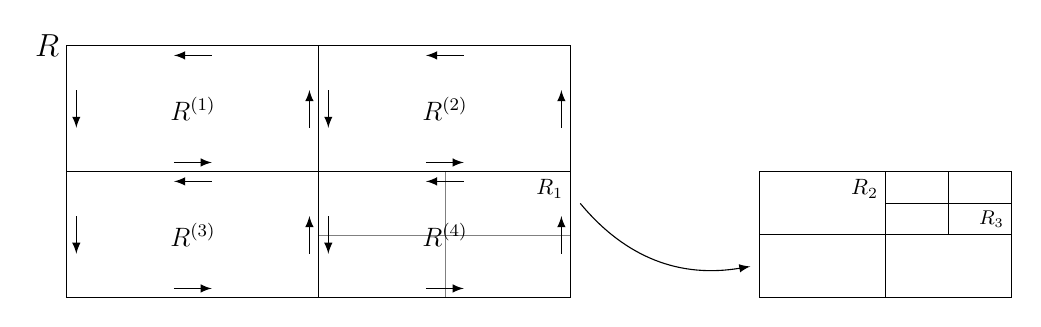
\begin{tikzpicture} [>=latex, scale=0.8, transform shape]
	\draw [help lines] (6,0) -- (6,2) (4,1) -- (8,1);
	\draw (0,0) rectangle (8,4);
	\draw (4,0) -- (4,4) (0,2) -- (8,2);
	\draw [->] (0.15,3.30) -- (0.15,2.70);
	\draw [->] (0.15,1.30) -- (0.15,0.70);
	\draw [->] (1.70,0.15) -- (2.30,0.15);
	\draw [->] (5.70,0.15) -- (6.30,0.15);
	\draw [<-] (7.85,3.30) -- (7.85,2.70);
	\draw [<-] (7.85,1.30) -- (7.85,0.70);
	\draw [<-] (1.70,3.85) -- (2.30,3.85);
	\draw [<-] (5.70,3.85) -- (6.30,3.85);
	\draw [->] (1.70,2.15) -- (2.30,2.15);
	\draw [->] (5.70,2.15) -- (6.30,2.15);
	\draw [<-] (1.70,1.85) -- (2.30,1.85);
	\draw [<-] (5.70,1.85) -- (6.30,1.85);
	\draw [->] (4.15,3.30) -- (4.15,2.70);
	\draw [->] (4.15,1.30) -- (4.15,0.70);
	\draw [<-] (3.85,3.30) -- (3.85,2.70);
	\draw [<-] (3.85,1.30) -- (3.85,0.70);
	\node [font=\large] at (2,3) {\(R^{(1)}\)};
	\node [font=\large] at (6,3) {\(R^{(2)}\)};
	\node [font=\large] at (2,1) {\(R^{(3)}\)};
	\node [font=\large] at (6,1) {\(R^{(4)}\)};
	\node [left, font=\Large] at (0,4) {\(R\)};
	\node [below left] at (8,2) {\(R_1\)};
	\draw [->] (8.15,1.5) to [bend right=30] (10.85,0.5);
	\draw (11,0) rectangle (15,2);
	\draw (13,0) -- (13,2) (11,1) -- (15,1);
	\draw (14,1) -- (14,2) (13,1.5) -- (15,1.5);
	\node [below left] at (13,2) {\(R_2\)};
	\node [above left, font=\small] at (15,1) {\(R_3\)};
\end{tikzpicture}
	\caption{Bisezione del rettangolo \(R\).}
	\label{fig:teorCauchyRettangolo}
\end{figure}

\begin{proof}
	Possiamo supporre che \(f\) sia olomorfa in un aperto che contiene \(R\). Infatti se prendo \(R_n \subseteq \mathring{R}\) con \(R_n \to R\), avrò che \(f\) è olomorfa in un aperto che contiene \(R_n\).
	Per il lemma precedente avremo
	\[
		\int\limits_{\pd R_n}f(z)\,\dd z = 0,\,\fa n \implies \int\limits_{\pd R}f(z)\,\dd z =0.
	\]
	Introduciamo la notazione
	\[
		\h(R) = \int\limits_{\pd R}f(z)\,\dd z,
	\]
	che utilizzeremo anche per ogni rettangolo contenuto in quello di partenza.
	Se dividiamo \(R\) in quattro rettangoli congruenti \(R^{(1)},R^{(2)},R^{(3)},R^{(4)}\), otteniamo che
	\[
		\h(R) = \h(R^{(1)})+\h(R^{(2)})+\h(R^{(3)})+\h(R^{(4)}),
	\]
	dal momento che, come è visibile nella \autoref{fig:teorCauchyRettangolo}, gli integrali si cancellano a vicenda sulle linee in comune.
	Applicando la triangolare avremo
	\[
		\abs{\h(R)} = \abs{\h(R^{(1)})+\h(R^{(2)})+\h(R^{(3)})+\h(R^{(4)})} \le \abs{\h(R^{(1)})}+\abs{\h(R^{(2)})}+\abs{\h(R^{(3)})}+\abs{\h(R^{(4)})},
	\]
	per cui almeno uno dei rettangoli \(R^{(k)}\), \(k=1,2,3,4\), soddisferà la condizione
	\[
		\abs{\h(R^{(k)})} \ge \frac{1}{4}\abs{\h(R)}.
	\]
	Chiamiamo tale rettangolo \(R_1\).
	Iterando questo processo otteniamo una catena di rettangoli \(R\supset R_1 \supset \ldots \supset R_n \supset ...\) con la proprietà
	\[
		\abs{\h(R_n)} \ge \frac{1}{4}\abs{\h(R_{n-1})} \implies \abs{\h(R_n)} \ge \frac{1}{4^n}\abs{\h(R)}.
	\]
	Poiché la catena di rettangoli è in particolare una catena di compatti, la loro intersezione convergerà ad un punto \(z^*\in R\), ovvero \(R_n\) sarà contenuto in un intorno \(D(z^*,\d)\) quando \(n\) sarà sufficientemente grande.
	Possiamo inoltre prendere \(\d\) abbastanza piccolo affinché \(f\) sia definita e olomorfa in \(D(z^*,\d)\).
	Inoltre, fissato \(\e>0\), possiamo trovare \(\d\) tale che
	\[
		\abs*{\frac{f(z)-f(z^*)}{z-z^*}-f'(z^*)} \le \e \qquad\text{se }\abs{z-z^*}<\d,
	\]
	ovvero
	\begin{equation}\label{eq:teorCauchyRettangoli}
		\abs{f(z)-f(z^*)-f'(z^*)(z-z^*)} \le \e\abs{z-z^*} \qquad\text{se }\abs{z-z^*}<\d.
	\end{equation}
	Assumiamo quindi che \(\d\) soddisfi queste condizioni e che \(R_n\) sia contenuto in \(D(z^*,\d)\).
	Osserviamo inoltre che
	\[
		\int\limits_{\pd R_n} \dd z = 0 \qquad\text{e}\qquad \int\limits_{\pd R_n} z\,\dd z = 0.
	\]
	Questi casi particolari sono banalmente veri in quanto \(1\) e \(z\) sono rispettivamente le derivate di \(z\) e \(z^2/2\) e \(\pd R_n\) è una curva chiusa.

	Di conseguenza possiamo scrivere
	\[
		\h(R_n) = \int\limits_{\pd R_n} f(z)\,\dd z = \int\limits_{\pd R_n} \big[f(z)-f(z^*)-f'(z^*)(z-z^*)\big]\,\dd z,
	\]
	da cui, per la \eqref{eq:teorCauchyRettangoli}
	\[
		\abs{\h(R_n)} \le \int\limits_{\pd R_n} \e\,\abs{z-z^*}\,\abs{\dd z}.
	\]
	Nell'ultimo integrale \(\abs{z-z^*}\) è al più uguale al diametro \(D_n\) di \(R_n\).
	Inoltre, se denotiamo con \(P_n\) il perimetro di \(R_n\), otteniamo
	\[
		\abs{\h(R_n)} \le \e\,D_n\,\int\limits_{\pd R_n} \abs{\dd z} = \e\,D_n P_n.
	\]
	D'altronde se \(D\) e \(P\) sono rispettivamente il diametro e il perimetro del rettangolo \(R\) di partenza, valgono
	\[
		D_n = \frac{D}{2^n} \qquad\text{e}\qquad P_n = \frac{P}{2^n},
	\]
	da cui
	\[
		\abs{\h(R_n)} \le \frac{\e\,D\,P}{4^n} \implies \abs{\h(R)} \le \e\,D\,P.
	\]
	Dal momento che \(\e\) è arbitrario possiamo solamente avere \(\h(R)=0\), ovvero la tesi.
\end{proof}

\begin{teor}{di Cauchy per i dischi aperti}{teorCauchyDischi}\index{Teorema di Cauchy!per i dischi aperti}
	Siano \(D\subseteq\C\) un disco aperto e \(z_0\) il centro di \(D\).
	Sia \(f\colon D \to \C\) olomorfa in \(D\).
	Se \(\g\colon [a,b] \to D\) è una curva chiusa di classe \(C^1\), allora
	\[
		\int\limits_\g f(z)\,\dd z = 0.
	\]
\end{teor}

\begin{figure}[tp]
	\centering
	\begin{tikzpicture}[>=To]
	\coordinate [label={[font=\large]below left:\(z_0\)}] (A) at (0,0);
	\coordinate (B) at (3,0);
	\coordinate (C) at (5,0);
	\coordinate (D) at (5,3);
	\coordinate [label={[font=\large]left:\(z\)}] (E) at (3,3);
	\coordinate [label={[font=\large]right:\(z+h\)}] (F) at (5,5);

	\draw [->-] (A) -- (B);
	\draw [->-] (B) -- (C);
	\draw [->-] (C) -- (D);
	\draw [->-, very thick] (D) -- (F);
	\draw [->-] (B) -- (E);
	\draw [->-, very thick] (E) -- (D);
	\draw (E) -- (F);

	\node [above=0.1cm] at ($(A)!0.5!(B)$) {\(\g_1\)};
	\node [left=0.1cm] at ($(B)!0.5!(E)$) {\(\g_2\)};
	\node [above=0.1cm] at ($(B)!0.5!(C)$) {\(\g_3\)};
	\node [right=0.1cm] at ($(C)!0.5!(D)$) {\(\g_4\)};
	\node [right=0.1cm] at ($(D)!0.5!(F)$) {\(\g_5\)};
	\node [below=0.1cm] at ($(D)!0.5!(E)$) {\(\g_6\)};
\end{tikzpicture}
	\caption{Curve per \(F(z+h)-F(z)\).}
	\label{fig:teorCacuhyDisco}
\end{figure}

\begin{proof}
	Per la \autoref{pr:integraleDerivataContinua} è sufficiente trovare \(F\colon D \to \C\) olomorfa tale che \(F'(z)=f(z),\,\fa z\in D\).
	Definisco quindi
	\[
		F(z) = \int\limits_{\g_1} f(w)\,\dd w + \int\limits_{\g_2} f(w)\,\dd w,
	\]
	dove \(\g_1\) consiste nella curva orizzontale da \((x_0,y_0)\) a \((x,y_0)\) e \(\g_2\) in quella verticale da \((x,y_0)\) a \((x,y)\).

	Per mostrare che \(F\) è olomorfa e vale \(F'(z)=f(z)\), per prima cosa mostriamo \(F'(z_0)=f(z_0)\), verificandolo con la definizione di derivata.
	Posto \(h=z-z_0\) avremo
	\[
		\begin{split}
			\bigg\lvert\frac{1}{h}\big[F(z)-\cancel{F(z_0)}-f(z_0)h\big]\bigg\rvert & = \bigg\lvert\frac{1}{h}\bigg[ \int\limits_{\g_1+\g_2}f(w)\,\dd w - f(z_0)h \bigg]\bigg\rvert = \bigg\lvert \frac{1}{h} \int\limits_{\g_1+\g_2}\big[f(w)-f(z_0)\big]\,\dd w \bigg\rvert\\
			& \le \frac{1}{\abs{h}} \int\limits_{\g_1+\g_2} \big\lvert f(w) - f(z_0) \big\rvert\,\abs{\dd w} \le \frac{\e}{\abs{h}} \int\limits_{\g_1+\g_2} \abs{\dd w}\graffito{\(\big\lvert f(w)-f(z_0)\big\rvert \le \e\) se \(\abs{h}<\d\)}\\
			& = \frac{\e}{\abs{h}}\,\sqrt{2}\abs{h} = \e \sqrt{2}
		\end{split}
	\]
	Per cui dato \(\e\) trovo \(\d\) tale che, per \(\abs{h}<\d\), si ha
	\[
		\bigg\lvert\frac{1}{h}\big[F(z)-F(z_0)-f(z_0)h\big]\bigg\rvert \le \e \implies F'(z_0) = f(z_0).
	\]
	Mostriamo adesso il caso generale:
	\[
		F(z+h)-F(z) = \int\limits_{\mathclap{\cancel{\g_1}+\g_3+\g_4+\g_5}}f(w)\,\dd w - \int\limits_{\mathclap{\cancel{\g_1}+\g_2}} f(w)\,\dd w,
	\]
	dove \(\g_1,\g_2,\g_3,\g_4,\g_5,\g_6\) sono le curve mostrate in \autoref{fig:teorCacuhyDisco}.
	Ora, il \hyperref[th:teorCauchyRettangoli]{teorema di Cauchy per i rettangoli} applicato al rettangolo identificato da \(\g_2+\g_6-\g_4-\g_3\) ci dice che l'integrale di \(f\) lungo il rettangolo è nullo, per cui
	\[
		\begin{split}
			F(z+h)-F(z) & = \int\limits_{\mathclap{\g_3+\g_4+\g_5}}\,f(w)\,\dd w - \int\limits_{\g_2}f(w)\,\dd w = \int\limits_{\mathclap{\g_3+\g_4+\g_5}}\,f(w)\,\dd w - \int\limits_{\g_2}f(w)\,\dd w + \int\limits_{\mathclap{\g_2+\g_6-\g_4-\g_3}}\,f(w)\,\dd w\\
			& = \int\limits_{\mathclap{\g_5+\g_6}}\,f(w)\,\dd w,
		\end{split}
	\]
	che è analogo al caso precedente.
\end{proof}